%%
%% This is file `sample-sigconf.tex',
%% generated with the docstrip utility.
%%
%% The original source files were:
%%
%% samples.dtx  (with options: `sigconf')
%% 
%% IMPORTANT NOTICE:
%% 
%% For the copyright see the source file.
%% 
%% Any modified versions of this file must be renamed
%% with new filenames distinct from sample-sigconf.tex.
%% 
%% For distribution of the original source see the terms
%% for copying and modification in the file samples.dtx.
%% 
%% This generated file may be distributed as long as the
%% original source files, as listed above, are part of the
%% same distribution. (The sources need not necessarily be
%% in the same archive or directory.)
%%
%% The first command in your LaTeX source must be the \documentclass command.
\documentclass[sigconf,review, anonymous]{acmart}
\acmConference[ISSTA 2020]{ACM SIGSOFT International Symposium on Software Testing and Analysis}{18–22 July, 2020}{Los Angeles, US}

\pagenumbering{arabic} % Remove for camera-ready

\usepackage{libertine}
\usepackage{lipsum}% http://ctan.org/pkg/lipsum
\usepackage{algorithm}% http://ctan.org/pkg/algorithm
\usepackage{algpseudocode}% http://ctan.org/pkg/algorithmicx
\usepackage{graphicx}
\usepackage[compatibility=false]{caption}% http://ctan.org/pkg/caption
\usepackage{booktabs}
%% \usepackage{cite}
\usepackage{url}
\usepackage{multirow}
\usepackage{pgfplots}
\usepackage{tikz}
\usetikzlibrary{matrix,fit,shapes,calc,positioning,shadows,arrows,shapes,backgrounds,decorations.markings,fadings}
\usepackage{listings}
\usepackage[caption=false, font=footnotesize]{subfig}
\renewcommand{\ttdefault}{pcr}
\lstset{
  basicstyle=\scriptsize\ttfamily,
  keywordstyle=\scriptsize\ttfamily\bfseries,
  language=C,             % choose the language of the code
  frame=single,              % adds a frame around the code
  aboveskip=0pt,
  belowskip=0pt,
  breaklines=true,           % sets automatic line breaking
  breakatwhitespace=false,   % sets if automatic breaks should only happen at
  showspaces=false,
  %numbersep=5pt,              % Abstand der Nummern zum Text
  %tabsize=2,                  % Groesse von Tabs
  %extendedchars=true,         %
  %breaklines=true,            % Zeilen werden Umgebrochen
  keywords=[2]{tcp, flag, threshold, track, count, seconds, classtype, sid}
}
\usepackage{balance}
\usepackage{wrapfig}
\usepackage{enumitem}
\usepackage{color, colortbl}
\definecolor{Gray}{gray}{0.9}

%% 
\newcommand{\tname}{\textsc{Syrius}} %% name of the technique
\newcommand{\ie}{i.e.}
\newcommand{\eg}{e.g.}
\newcommand{\aka}{a.k.a.}
\newcommand{\etal}{and colleagues}
\newcommand{\nids}{NIDS}
\newcommand{\metas}{Metasploit}
\newcommand{\suri}{Suricata}
\newcommand{\numrulessuri}{27.8K}
\newcommand{\percRulesWithContent}{93.5\%}
\newcommand{\numundetected}{\Fix{XX\%}}
\newcommand{\CodeIn}[1]{{\small{\texttt{#1}}}}
\newcommand{\MyComment}[1]{}

%% review
\newcommand{\Fix}[1]{{\textbf{[[}\color{magenta}#1}\textbf{]]}}
\newcommand{\Mar}[1]{{\textbf{[[Marcelo:~}\color{red}#1}\textbf{]]}}
\newcommand{\Luc}[1]{{\textbf{[[Lucas:~}\color{blue}#1}\textbf{]]}}
\newcommand{\Gui}[1]{{\textbf{[[Guilherme:~}\color{green}#1}\textbf{]]}}

\def\denseitems{
   \itemsep1pt plus1pt minus1pt
   \parsep0pt plus0pt
   \parskip0pt\topsep0pt}

%% numbers
\newcommand{\totoptions}{162}
\newcommand{\numproto}{11}
\newcommand{\totoptionsrelevant}{153}


%%
%% \BibTeX command to typeset BibTeX logo in the docs
\AtBeginDocument{%
  \providecommand\BibTeX{{%
    \normalfont B\kern-0.5em{\scshape i\kern-0.25em b}\kern-0.8em\TeX}}}

%% Rights management information.  This information is sent to you
%% when you complete the rights form.  These commands have SAMPLE
%% values in them; it is your responsibility as an author to replace
%% the commands and values with those provided to you when you
%% complete the rights form.
%% \setcopyright{acmcopyright}
%% \copyrightyear{2018}
%% \acmYear{2018}
%% \acmDOI{10.1145/1122445.1122456}

%% These commands are for a PROCEEDINGS abstract or paper.
%% \acmConference[Woodstock '18]{Woodstock '18: ACM Symposium on Neural
%%   Gaze Detection}{June 03--05, 2018}{Woodstock, NY}
%% \acmBooktitle{Woodstock '18: ACM Symposium on Neural Gaze Detection,
%%   June 03--05, 2018, Woodstock, NY}
%% \acmPrice{15.00}
%% \acmISBN{978-1-4503-XXXX-X/18/06}


%%
%% Submission ID.
%% Use this when submitting an article to a sponsored event. You'll
%% receive a unique submission ID from the organizers
%% of the event, and this ID should be used as the parameter to this command.
%%\acmSubmissionID{123-A56-BU3}

%%
%% The majority of ACM publications use numbered citations and
%% references.  The command \citestyle{authoryear} switches to the
%% "author year" style.
%%
%% If you are preparing content for an event
%% sponsored by ACM SIGGRAPH, you must use the "author year" style of
%% citations and references.
%% Uncommenting
%% the next command will enable that style.
%%\citestyle{acmauthoryear}

%%
%% end of the preamble, start of the body of the document source.
\begin{document}

%%
%% The "title" command has an optional parameter,
%% allowing the author to define a "short title" to be used in page headers.
\title{Learning to Synthesize Rules for Network Intrusion Detectors}

%%
%% The "author" command and its associated commands are used to define
%% the authors and their affiliations.
%% Of note is the shared affiliation of the first two authors, and the
%% "authornote" and "authornotemark" commands
%% used to denote shared contribution to the research.
\author{Ben Trovato}
\authornote{Both authors contributed equally to this research.}
\email{trovato@corporation.com}
\orcid{1234-5678-9012}
\author{G.K.M. Tobin}
\authornotemark[1]
\email{webmaster@marysville-ohio.com}
\affiliation{%
  \institution{Institute for Clarity in Documentation}
  \streetaddress{P.O. Box 1212}
  \city{Dublin}
  \state{Ohio}
  \postcode{43017-6221}
}

\author{Lars Th{\o}rv{\"a}ld}
\affiliation{%
  \institution{The Th{\o}rv{\"a}ld Group}
  \streetaddress{1 Th{\o}rv{\"a}ld Circle}
  \city{Hekla}
  \country{Iceland}}
\email{larst@affiliation.org}

\author{Valerie B\'eranger}
\affiliation{%
  \institution{Inria Paris-Rocquencourt}
  \city{Rocquencourt}
  \country{France}
}

\author{Aparna Patel}
\affiliation{%
 \institution{Rajiv Gandhi University}
 \streetaddress{Rono-Hills}
 \city{Doimukh}
 \state{Arunachal Pradesh}
 \country{India}}

\author{Huifen Chan}
\affiliation{%
  \institution{Tsinghua University}
  \streetaddress{30 Shuangqing Rd}
  \city{Haidian Qu}
  \state{Beijing Shi}
  \country{China}}

\author{Charles Palmer}
\affiliation{%
  \institution{Palmer Research Laboratories}
  \streetaddress{8600 Datapoint Drive}
  \city{San Antonio}
  \state{Texas}
  \postcode{78229}}
\email{cpalmer@prl.com}

\author{John Smith}
\affiliation{\institution{The Th{\o}rv{\"a}ld Group}}
\email{jsmith@affiliation.org}

\author{Julius P. Kumquat}
\affiliation{\institution{The Kumquat Consortium}}
\email{jpkumquat@consortium.net}

%%
%% By default, the full list of authors will be used in the page
%% headers. Often, this list is too long, and will overlap
%% other information printed in the page headers. This command allows
%% the author to define a more concise list
%% of authors' names for this purpose.
\renewcommand{\shortauthors}{Trovato and Tobin, et al.}

%%
%% The abstract is a short summary of the work to be presented in the
%% article.
\begin{abstract}
Network Intrusion Detection Systems (\nids{}) are a popular mechanism
used by system administrators to defend against network attacks. These
systems monitor the network traffic and flag suspicious network
behavior. Signature-based \nids\ do that by checking the network
traffic against a pre-defined set of rules, which can become obsolete
as attackers learn new strategies to circumvent existing defenses.
This paper proposes \tname{}, a technique that automatically
synthesizes \nids\ rules from positive and negative examples, \ie{},
malicious and benign traffic. \tname{} formulates synthesis as an
optimization problem whose candidate solutions are rules that maximize
the capture of positive traffic and minimize the capture of negative
traffic. \tname{} bootstraps the search with candidate solutions that
use data from the payload of the malicious message and produces
optimal rule candidates on output. We evaluated \tname{} on a diverse
set of attacks. Results indicate that \Fix{...}
\end{abstract}

%%
%% The code below is generated by the tool at http://dl.acm.org/ccs.cfm.
%% Please copy and paste the code instead of the example below.
%%
\begin{CCSXML}
<ccs2012>
 <concept>
  <concept_id>10010520.10010553.10010562</concept_id>
  <concept_desc>Computer systems organization~Embedded systems</concept_desc>
  <concept_significance>500</concept_significance>
 </concept>
 <concept>
  <concept_id>10010520.10010575.10010755</concept_id>
  <concept_desc>Computer systems organization~Redundancy</concept_desc>
  <concept_significance>300</concept_significance>
 </concept>
 <concept>
  <concept_id>10010520.10010553.10010554</concept_id>
  <concept_desc>Computer systems organization~Robotics</concept_desc>
  <concept_significance>100</concept_significance>
 </concept>
 <concept>
  <concept_id>10003033.10003083.10003095</concept_id>
  <concept_desc>Networks~Network reliability</concept_desc>
  <concept_significance>100</concept_significance>
 </concept>
</ccs2012>
\end{CCSXML}

\ccsdesc[500]{Computer systems organization~Embedded systems}
\ccsdesc[300]{Computer systems organization~Redundancy}
\ccsdesc{Computer systems organization~Robotics}
\ccsdesc[100]{Networks~Network reliability}

%%
%% Keywords. The author(s) should pick words that accurately describe
%% the work being presented. Separate the keywords with commas.
\keywords{\nids, synthesis, search}

%% This command processes the author and affiliation and title
%% information and builds the first part of the formatted document.
\maketitle

\section{Introduction}
\label{sec:intro}

Network Intrusion Detection Systems (\nids{}) are software systems
that monitor the network traffic for malicious behavior and act
accordingly by blocking messages or alerting humans about suspicious
events~\cite{Mitchell:2014:SID:2597757.2542049}. \nids{} are typically
placed behind a firewall, vetting the traffic that the firewall did
not block. Various open-source (\eg{}, Snort~\cite{snort} and
Suricata~\cite{suricata}) and commercial \nids\ implementations (\eg{},
SolarWinds~\cite{solarwinds} and IBM QRadar~\cite{qradar}) exist
today. These systems are very popular in industry to secure local
computer networks given the amount of potential malicious traffic that
exist on the Internet.

This paper focuses on rule-based \nids{}, which is a very popular kind
of NIDS used in industry (see Section~\ref{sec:background}). A
\emph{rule-based intrusion detector}\footnote{\aka\ signature-based
  intrusion detector.} checks if the network traffic matches a fixed
set of rules. Figure~\ref{fig:synflood-example} shows an example rule
of Suricata~\cite{suricata}, a popular open-source \nids{}. This
particular rule prescribes a method to capture a denial-of-service
attack to a server by matching specific conditions about the network
traffic~\cite{understanding-dos}. Relevant properties about the
traffic of interest appear in bold in this rule (see
Section~\ref{sec:suri-metas-coverage}). Deployments of rule-based
\nids\ are restricted to a fixed set of rules defined by the network
system administrator. Updating these rules is tedious and error-prone,
but it is important as attackers constantly create new strategies to
circumvent existing rules. IT-security companies capitalize on this
phenomena and offer rulesets on the
market~\cite{proofpoint-etpro,snort-rule-subscriptions}.

This paper proposes \tname{}\footnote{Abbreviation for
  \textbf{Sy}nthesis of Su\textbf{ri}cata R\textbf{u}le\textbf{s}.}, a
technique that uses machine intelligence to automatically synthesize
rules for rule-based \nids. Our goal is to facilitate the creation
process of rules and, consequently, harden the protection of \nids\ to
network attacks. \tname{} synthesizes rules from malicious and benign
traffic and from examples of correct rules.

%% Note that anomaly-based \nids are evolving pretty quick with the
%% advances in machine learning, but rule-based \nids are still extremely
%% popular.  \tname{} could also leverage existing databases of malicious
%% traffic to synthesize rules.  Regardless of how the negative traffic
%% is produced (out of scope of this paper), those rules can be
%% distributed to rule databases for free.
%%  The
%% core motivation is that 1) attackers are productive in creating new
%% ways to circumvent existing protections and 2) manual creation of
%% rules is tedious and time-consuming.  

\Fix{summarize how the technique works}

\Fix{summarize results}

This paper makes the following contributions.

\section{Network Intrusion Detection Systems (\nids)}
\label{sec:background}

\subsection{Rule-based and Anomaly-based \nids}

\sloppy \nids{} are typically categorized in two
groups~\cite{kumar2007survey}: rule-based (see
Section~\ref{sec:intro}) and anomaly-based \nids. An
\emph{anomaly-based intrusion detector} learn usage behavior from
benign traffic and, based on that, alert uncommon
behavior~\cite{7579764,kumar2007survey,Mitchell:2014:SID:2597757.2542049,cordy-etal-issta19}. More
precisely, an anomaly-based \nids{} flags an attack when the network
traffic manifests different characteristics compared to those of the
benign traffic.

Rule-based \nids\ can miss attacks as rulesets can become outdated
whereas anomaly-based \nids\ can report false alarms as learning
algorithms that generalize observations from bening traffic are
approximate. To sum up, rule-based \nids{} and anomaly-based \nids{}
are complementary---a rule-based \nids{} focuses on known attacks
whereas anomaly-based \nids{} focuses on unknown potential attacks.
This paper focuses on rule-based \nids\ for its tremendous popularity
in industry. Although we focused on the Suricata \nids, the principles
we used are general to any other signature-based \nids~(\eg{},
Snort~\cite{snort}).


\subsection{Suricata Rules}
\label{sec:example-suricata-rules}

Figure~\ref{fig:synflood-example} shows an example rule of
Suricata~\cite{suricata}, a popular open-source \nids{} maintained by
the Open Information Security Foundation (OISF)~\cite{oisf}. A
Suricata rule is divided in three parts---action, header, and rule
options~\cite{suri-rule-format}. The action part appears as the first
word in the rule description. An action denotes the task that needs to
be executed if the rule pattern is satisfied. In this example, a
message will be sent to system administrators if the rule pattern is
satisfied. The header comes after the action in the rule
description. It restricts the information flow covered by the
rule. For this rule, the header is \CodeIn{tcp \$HOME\_NET any ->
  \$EXTERNAL\_NET any}. It instructs Suricata to inspect \CodeIn{tcp}
traffic flowing from any port in the home network to any other address
outside the home network. The variables \CodeIn{\$HOME\_NET} and
\CodeIn{\$EXTERNAL\_NET} are configurable. The rule options come after
the header. It is a semi-colon-separated sequence of key-value
pairs. Rule options serve to document the analyzed traffic (\eg{},
``msg'', ``classtype'', and ``sid'') and to characterize the attack
pattern (\eg, ``flags'', ``threshold'', and ``content''). \tname{}
produces options of the second kind, which are \emph{relevant} to
capturing the attack.

\begin{table}[t!]
  \caption{\label{table:rules}Example options of Suricata.}  
  \centering
  \begin{tabular}{clp{5.5cm}}
    \toprule
    \multicolumn{1}{c}{\#} & \multicolumn{1}{c}{Name} &  \multicolumn{1}{c}{Description}\\
    \midrule     
    1 & dsize & matches on the size of the packet payload\\
    2 & itype &  matches on a specific ICMP type\\
    3 & icode & matches on a specific ICMP code\\
    4 & icmp\_seq  & checks a ICMP sequence number\\
    5 & icmp\_id & matches on specific ICMP id-values\\
    6 & window & checks the size of the TCP window\\
    7 & flags & matches on TCP flags\\
    8 & fragbits & checks if the fragmentation or reserved bits are set in the IP header\\
    9 & threshold & controls the rule’s alert frequency\\
    10 & content & checks if argument is present on the payload\\
    \bottomrule
  \end{tabular}
\end{table}



Table~\ref{table:rules} shows a sample of the options of
Suricata. Column ``\#'' shows the option number, column ``Name'' shows
the name of the option, and column ``Description'' presents a short
description of the option purpose. We found that the option
\CodeIn{content} is particularly prevalent in rules from public
databases\MyComment{ (see Figure~\ref{fig:distribution-contents})}. This
option takes a sequence of bytes as argument (\eg{},
\CodeIn{content:''SELECT ''}) and checks if that sequence is present
in the payload of the message. Detailed description of the Suricata
rules can be found elsewhere~\cite{suri-rule-format}. It is worth
noting that Suricata supports a total of \totoptions\ distinct options
covering \numproto\ distinct protocols. A total of 9 of these options
are for documentation.\MyComment{For instance, the purpose of rule
  option \CodeIn{msg} is to print on the output an informative message
  indicating what kind of intrusion has been observed.}
Figure~\ref{fig:distribution-rules-protocol} shows the distributions
of these options per protocol. The sum of the number of protocol
options is higher than \totoptions\ as some options are shared across
different protocols. \tname{} does not make distinction among protocols.


%\begin{wrapfigure}[14]{r}{0.5\textwidth}
\begin{figure}[t!]
  \centering
%  \vspace{-7ex}
  \scalebox{0.85}{
    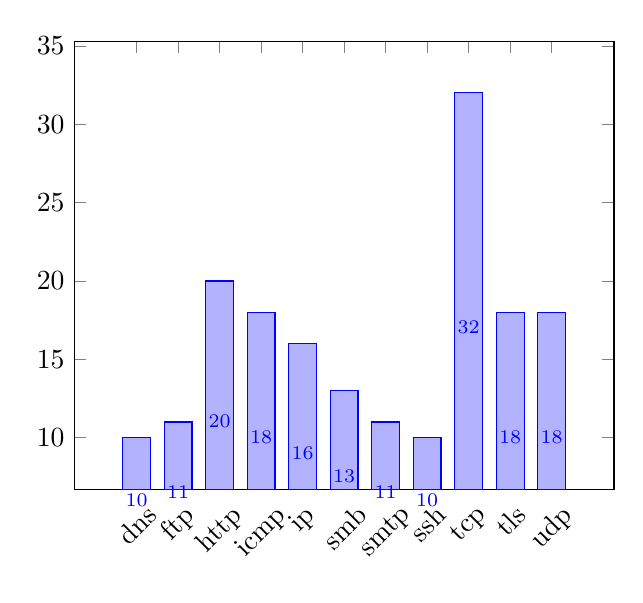
\begin{tikzpicture}
      \begin{axis}[
          ybar stacked,
          enlargelimits=0.15,
          legend style={at={(0.5,-0.15)},
            anchor=north,legend columns=-1},
          %          ylabel={\#rules},
          symbolic x coords={dns, ftp, http, icmp, ip, smb, smtp, ssh,
          tcp, tls, udp},
          xtick=data,
          xticklabel style={rotate=45},          
          nodes near coords,
          every node near coord/.append style={font=\scriptsize},        
          nodes near coords align={vertical},
        ]
        \addplot coordinates {(dns,10) (ftp,11) (http,20) (icmp,18)(ip,16) (smb,13) (smtp,11) (ssh, 10) (tcp, 32) (tls,18) (udp, 18)};
%        \legend{relevant, irrelevant}
      \end{axis}
    \end{tikzpicture}
  }
  \vspace{-2ex}
  \caption{\label{fig:distribution-rules-protocol}Number of relevant
    options per protocol supported by Suricata.}
%\end{wrapfigure}
\end{figure}
  

\subsection{Rules and Packets}
\label{sec:rules-and-packets}

\begin{figure}[h!]
\centering
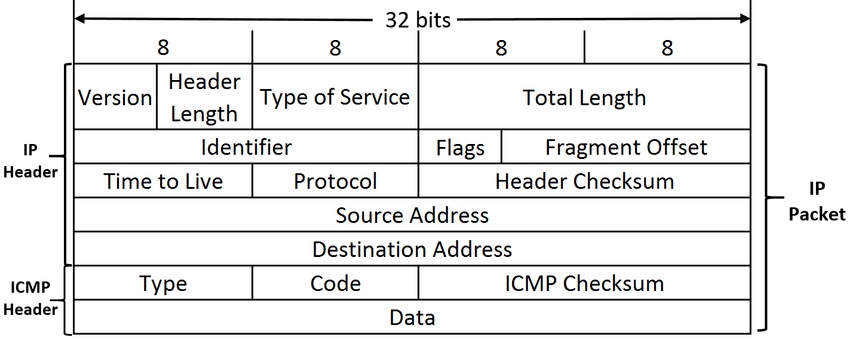
\includegraphics[scale=0.28]{figs/ICMP-packet-structure.png}
\caption{Layout of an ICMP packet.}
\label{fig:icmp-packet-layout}
\end{figure}

Rule options are often associated with specific fields of network
packets. Let's consider the ICMP protocol as an
example. Figure~\ref{fig:icmp-packet-layout} shows the layout of an
ICMP packet. The packet fields ``Flags'' and ``Time to Live'',
declared in the IP header, are mapped to the options \CodeIn{flagbits}
and \CodeIn{ttl}, respectively. Likewise, the fields ``Type'' and
``Code'', declared in the ICMP header, are mapped to the options
\CodeIn{itype} and \CodeIn{icode}. (Table~\ref{table:rules} lists some
example rule options.) The values of the options ``ttl'', ``itype'',
and ``icode'' are the same as the value of the corresponding fields in
the ICMP packet. For the field ``Flags'' the value of the
corresponding option is encoded in the bitvector. For example, if the
``Flags'' field stores the value 1010, the corresponding rule option
will be \CodeIn{flagbits:RM}, as each position of the vector encodes a
different character in the \CodeIn{flagbits} rule option. The value of
several options can be determined through transformation functions, as
those described above. One expection to this is the option
\CodeIn{threshold}, which is typically used in denial-of-service
attacks. That option operates over sequence of messages as opposed to
a single message. Consequently, it is not possible to determined its
values from a single message. More precisely, to trigger an action on
a rule containing that option a \nids\ tool needs to monitor several
messages.

%% \Luc{
%%   Os campos Flags e Time to live no header IP são mapeados para as opções fragbits e ttl, respectivamente. Os campos Type e Code no header ICMP são mapeados para as opções itype e icode. \\
%% Os campos, Time to Live, Type e Code recebem diretamente o valor que está no pacote. Por exemplo, se o campo Type no pacote possuir valor 8, na regra ele vai aparecer como itype:8.\\
%% O campo Flags é intepretado como um vetor de bits, onde cada posição representa uma flag. Na regra, o valor do campo Flags é traduzido em caracteres que representam cada flag presente no pacote. Por exemplo: se o campo Flags possuir o valor 1010, na regra aparecerá fragbits:RM, pois os caracteres R e M indicam a presença do quarto e segundo bits.}


\section{Illustrative Examples}
\label{sec:suri-metas-coverage}

This section briefly presents examples of attacks and illustrates the
rules that \tname{} synthesizes to capture those attacks.


\subsection{Denial-of-Service}
\label{sec:dos}

The SYN Flood attack is a denial-of-service attack that exploits a vulnerability in the TCP/IP handshake
to establish a TCP connection~\cite{cloudfare-synflood}. The handshake
works as follows in normal circumstances. First, a client sends a SYN
packet to the server, requesting a connection. Second, the server
responds with a SYN-ACK packet to the client. Third, the client
responds with an ACK message and the connection is established. Aware
of the protocol, an attacker sends multiple SYN packets to different
ports of a server, often using fake IP addresses. Then, after the
server responds with a SYN-ACK packet, the client keeps sending other
SYN packets to avoid the connection to time out. Without proper
protection, the server accepts these malicious requests and eventually
legitimate requests cannot be satisfied due to resource exhaustion.

\begin{figure}[h!]
  \lstinputlisting[language=C,numbers=none,keywords={flags,threshold}]{synflood.suricata}
  \caption{Suricata rule for SYN Flood Attacks.}
  \label{fig:synflood-example}
\end{figure}


Figure~\ref{fig:synflood-example} shows a Suricata rule that captures
this attack. This rule was obtained from the Emerging Threats Open
Ruleset~\cite{emerging-threats-open}. The relevant options in the
rule appear in bold---the option \CodeIn{flags: S,12}, identifies a
SYN packet in a TCP packet and the option \CodeIn{threshold: type
  both, track by\_dst, count 5000, seconds 5} indicates that a high
volume of such packets should be requested in a short period of time.

In the following, we illustrate how \tname{} proceeds for obtaining
the rule for the SYN Flood attack. The challenge in synthesizing rules
is to discover the set of options in a rule that makes the \nids\ to
capture the malicious traffic, but allow the benign traffic to go
through.  The other parts of the rule (\ie{}, the action and the
header) are either inferred or left constant. For example, in this
case, \tname{} sets the action header to \CodeIn{alert} and sets the
header to \CodeIn{<proto> any any -> any any}, indicating that it
infers the target protocol and uses the most general flow description
possible, \ie{}, it instructs the \nids\ to analyze the traffic
flowing from/to any address and port.  We understand that this is
domain-specific information and assume that the system administrator
would know how to customize it.

\tname{} proceeds as follows to synthesize rules for this
attack. First, it analyzes the positive (\ie, malicious) traffic and
extracts options expressed in that traffic. In this case, the
malicious traffic is characterized as a sequence of 20
messages. \tname{} finds the following set of options at this stage:

\begin{figure}[h]
  \vspace{-2ex}
  \lstinputlisting[language=C,numbers=none,frame=none,keywords={flags,threshold,window}]{synflood.suricata.synth}
%  \caption{Suricata rule for SYN Flood Attacks.}
  %  \label{fig:synflood-example-synt}
  \vspace{-2ex}  
\end{figure}

%% \Mar{@Lucas/Guilheme, há algo o que remover? talvez ``window:64''?
%%   Qual a correspondencia de ``flags:S,12'' com ``flags:S''? Por favor,
%%   respondam isto logo.}  \Gui{O window:64 seria removido
%%   sim.}\Mar{ok. vou explicar isto.}
  %% \Luc{O segundo campo da opção flags define flags que serão
  %%   ignoradas. Nesse caso a regra procura por pacotes onde apenas a
  %%   flag S está 'setada', independentemente do valor das flags 1 e
  %%   2. Portanto a regra gerada pode capturar coisas diferentes da
  %%   regra original. A inferencia do "12" n pode ser feita apenas a
  %%   partir do pacote de entrada, precisariamos tratar
  %%   isso.}\Mar{vc. pode explicar isto **mais detalhadamente** \Luc{a opção flags pode ter dois campos separados por virgula (ex: flags:S,12). o primeiro campo indica quais flags devem estar ativas em um pacote para que o suricata gere um alerta. se uma ou mais flags forem irrelevantes para a detecção de um determinado ataque (ou seja, se n importa se a flag está ou não ativa), elas serão adicionadas ao segundo campo.} E (1)
  %%   explicar que isto eh uma limitacao \Luc{n entendi exatamente oq explicar aqui.} e (2) indicar a possivel consequencia
  %%   disto? \Luc{a consequencia sao possiveis falsos negativos. ao não incluir flags no segundo campo podemos descartar pacotes por conta da presença de flags q n são relevantes (ou seja, vamos levar em conta flags q n deveriam interferir na detecção).}}

\noindent
\tname{} only reports a rule if the \nids\ instantiated with that rule
is able to capture the traffic passed on input. Consequently, by
construction, a rule that uses this set of options captures the
malicious traffic. Unfortunately, this rule is potentially
overspecified. Informally, the rule includes ``too specific''
characteristics of the malicious traffic and could potentially result
in false negatives. For example, in this particular case, note that
the option \CodeIn{windows: 64} is not included in the golden rule
from Figure~\ref{fig:synflood-example}.

Second, \tname{} uses negative (\ie{}, benign) traffic to mitigate the
overfitting issue. In this step, \tname{} searches for alternative
rules that preserves the invarianxt that a rule should capture the
positive traffic but not capture the negative traffic. It uses the
rule obtained in the previous step, containing three options, to
bootstrap the search for rules. The search generates rules containing
subsets of the options from the seed rule.

 
%% \Luc{Ataque "JBoss JMX Console Beanshell Deployer WAR Upload and Deployment Exploit"
%% . O payload do pacote é o seguinte:
%% \begin{figure}[H]
%%   \lstinputlisting[language=C,numbers=none,keywords={dsize,itype}]{adaptor-rule.suricata}
%%   \label{fig:rule-example}
%% \end{figure}

%% A partir disso produzimos uma regra com os seguintes contents:

%% \begin{figure}[H]
%%   \lstinputlisting[language=C,numbers=none,keywords={dsize,itype}]{adaptor-contents-splitted.suricata}
%%   \label{fig:rule-example}
%% \end{figure}

%% Depois da etapa da minimização, as top 5 regras são:

%% \begin{figure}[H]
%%   \lstinputlisting[language=C,numbers=none,keywords={dsize,itype}]{adaptor-top5-rules.suricata}
%%   \label{fig:rule-example}
%% \end{figure}

%% A regra de ouro é:

%% \begin{figure}[H]
%%   \lstinputlisting[language=C,numbers=none,keywords={dsize,itype}]{adaptor-golden-rule.suricata}
%%   \label{fig:rule-example}
%% \end{figure}

%% }

Finally, \tname{} ranks the inferred rules according to heuristics
extracted from a database of existing rules. One example heuristic
function we used to rank the generated rules was
\Fix{...elaborate...}. The list below shows the rule options for the
top-5 rules \tname{} produces for this attack.

\Mar{listem 5 primeira regras neste caso}

To sum up, \tname{} uses the messages that manifest an attack in the
first step (to create an overspecific seed rule), benign traffic in
the second step (to create a set of plausible rules from the seed
rule), and existing rules from popular sources in the third step (to
rank the generated rules).

\vspace{1ex}
\noindent
\textbf{Differences.}~Note that there are differences between the
options produced in the first step of \tname{} and the options from
the golden rule, as per Figure~\ref{fig:synflood-example}. The option
\CodeIn{flags} does not mention parameters \CodeIn{1 2}, there is an
extra option \CodeIn{window}, and there are differences in the option
\CodeIn{threshold}. Considering the option \CodeIn{flags}, the first
parameter of that option indicates what flags in the packet must be
set while the second parameter indicates non-mandatory flags (\ie{},
``don't cares''). The option \CodeIn{flags: S} indicates that the flag
``S'' must be set and all flags not mentioned (``1'' and ``2'', in our
case) must be unset for the \nids\ to capture the
traffic. Consequently, that choice of option alone could result in
false negatives and false positives. An attack that satisfies all
other conditions in a rule and have flags ``1'' or ``2'' set would be
captured by the original rule but not the inferred rule---a case of
false negative. Likewise, an attack that satisfies all conditions and
have flags ``1'' and ``2'' unset would be captured by the inferred
rule but not the original rule---a case of false positive. The set of
positive examples is to blame in this case. To mitigate this issue,
the input messages should have covered cases with options ``1'' or
``2'' set. Considering option \CodeIn{windows: 64}, \tname{} is able
to generate rules without that option, as discussed above. Considering
option \CodeIn{threshold}, the values used in the golden rule are
domain-specific. \tname{} uses default values for these options. We
conjecture that the system administrator would be able to configure
this option.


\subsection{Active Reconnaissance}
\label{sec:active-recon}

%% \Mar{@Lucas, acima falamos de porta. Abaixo nao falamos de
%%   porta, apenas de maquina. Vc. pode ser mais especifico? ->} \Luc{De
%%   fato estamos falando de duas coisas diferentes, mas ambas são
%%   exemplos de 'active reconnaissance'. Primeiramente citamos o port
%%   scanning, q tem o objetivo de encontrar portas abertas em uma
%%   maquina especifica. Depois falamos do ping scan, q tem o objetivo de
%%   encontrar ip's ativos numa rede.}


Active reconnaissance is a method used by malicious individuals to
collect information about a computing system to determine potential
vulnerabilities. Active reconnaissance is a preliminary step towards
an actual attack. For example, Ping Scan is a very common type of
attack that scans the network for IPs of accessible hosts. An attacker
sends several ICMP Echo requests to a range of IP addresses in the
network and checks which ones respond to the requests. This allow the
attacker to know which machines are active in the network. Then (s)he
can choose one of them to attack.

\begin{figure}[h!]
  \vspace{1ex}
  \lstinputlisting[language=C,numbers=none,keywords={dsize,itype}]{pingscan.suricata}
  \caption{Suricata rule for Ping Scan.}
  \label{fig:pingscan-example}
  \vspace{1ex}  
\end{figure}

\begin{figure*}[ht!]
  \centering
  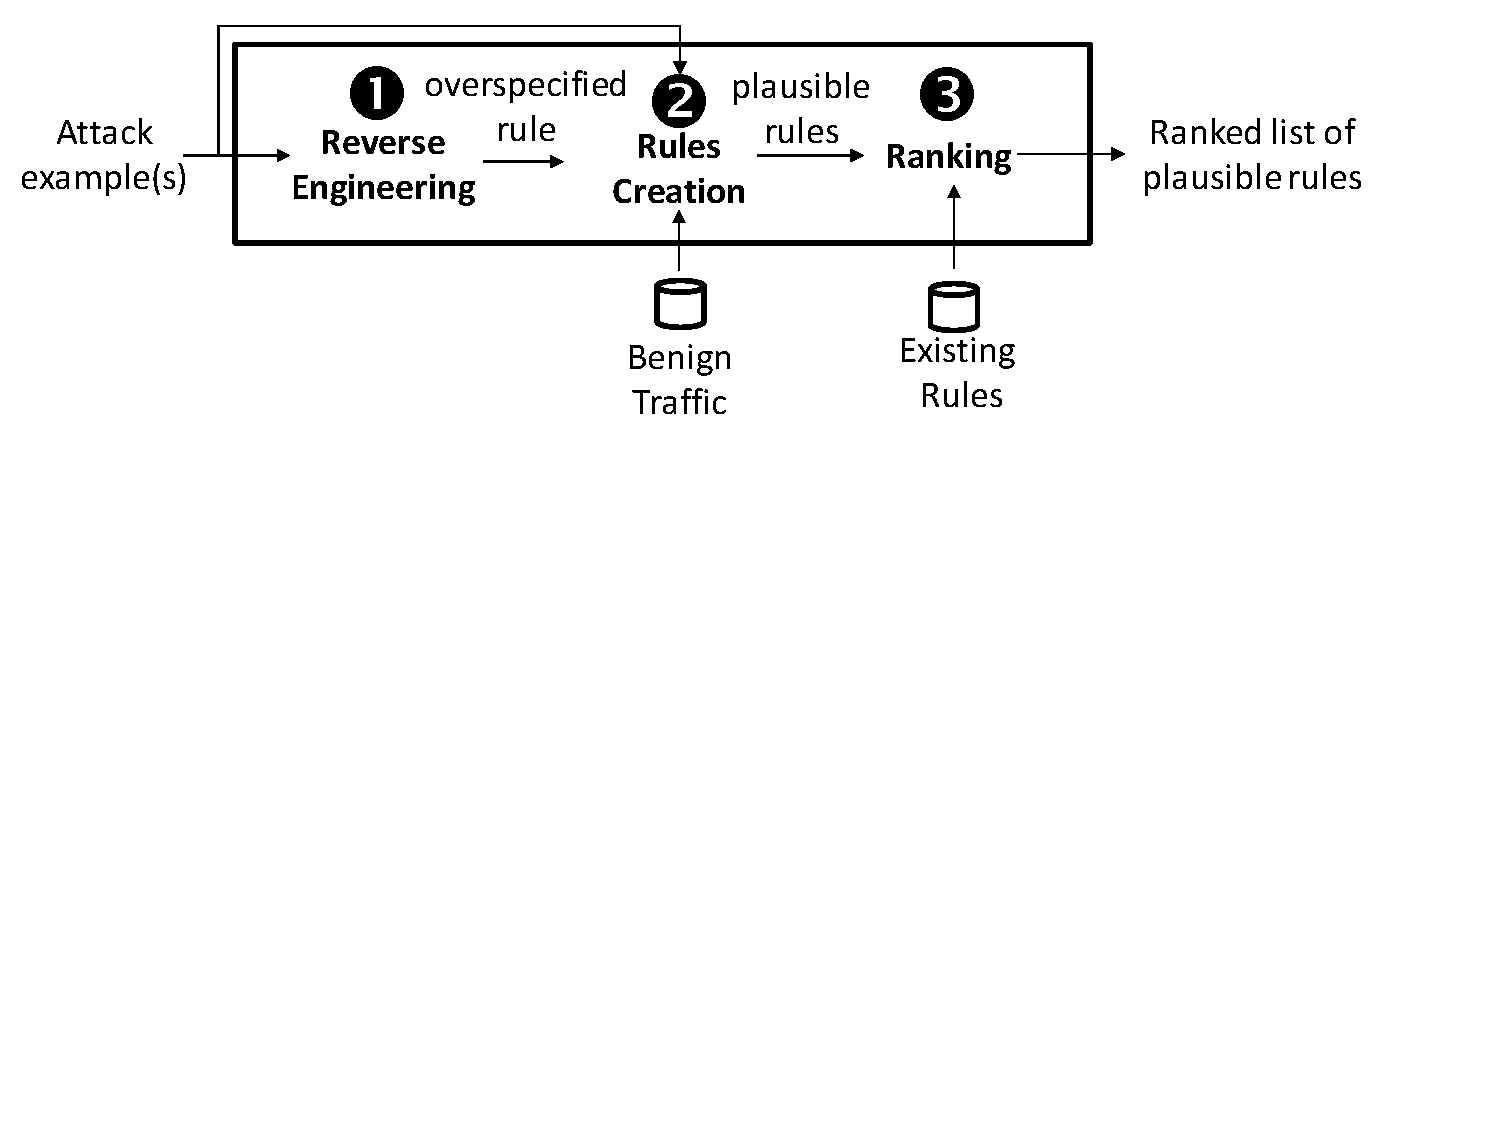
\includegraphics[trim=0 350 100 0,clip,width=0.65\textwidth]{figs/nids-workflow}
  \caption{\tname\ workflow.}
  \label{fig:overview}
  \vspace{-1ex}
\end{figure*}


Figure 4 shows a Suricata rule that captures a reproduction of a Ping
Scan attack available from NMAP~\cite{netmap}, a network discovery and
security auditing open-source tool. The relevant options are in
bold---the option \CodeIn{dsize: 0} indicates that the packet has no
bytes in the payload and the option \CodeIn{itype: 8} indicates that
the packet to be captured are ICMP Echo requests.

Again, to synthesize rules for a Ping Scan, \tname{} analyzes the
positive malicious traffic and extracts the following rule options:

\begin{figure}[h]
  \vspace{-2ex}
  \lstinputlisting[language=C,numbers=none,frame=none,keywords={dsize,icode,itype,icmp\_id,icmp\_seq}]{pingscan.suricata.synth}
  \vspace{-3ex}  
\end{figure}


Again, note that rule \CodeIn{icode} was not present in the original
rule.  \tname{} produces the following five rules at the top of the
ranking after minimization and ranking.

\begin{figure}[h]
  \vspace{-2ex}
  \lstinputlisting[language=C,numbers=none,frame=none,keywords={dsize,icode,itype,icmp\_id,icmp\_seq}]{top-pingscan.rules}
  \vspace{-3ex}  
\end{figure}

\Luc{Apenas 3 regras tiveram f1 de 100\%. O total de regras nesse caso foi de 13.}
\Fix{...listem 5 primeiras regras neste caso...}


\subsection{Remote Code Execution}
\label{sec:rce}

\Luc{"RCE refers to the process by which an agent can exploit a network vulnerability to run arbitrary code on a targeted machine or system. In an RCE attack, hackers intentionally exploit a remote code execution vulnerability to run malware. By prompting the targeted device to perform code execution, a hacker can run their own programming in its place. This programming can then enable them to gain full access, steal data, carry out a full distributed denial of service (DDoS) attack, destroy files and infrastructure, or engage in illegal activity. And as the term remote execution suggests, an RCE cyberattack can take place from any geophysical location."\\ Texto copiado de:  https://www.solarwindsmsp.com/blog/remote-code-execution \\
---------------- estou aqui}

\Mar{Note que a gente organizou estas secoes por tipo de ataque. Este
  titulo eh muito especifico.}
\Luc{JBoss é um servidor de aplicação Java muito popular, de codigo aberto. Esse ataque tem como alvo esses servidores e permite que seja feita execução remota de comandos. Os pacotes que estamos utilizando para testar esse ataque foram gerados pelo Nikto, mas o Metasploit tambem possui um modulo para ele. A regra de ouro para esse ataque é:

\begin{figure}[H]
  \lstinputlisting[language=C,numbers=none,keywords={content}]{adaptor-golden-rule.suricata}
  \label{fig:rule-example}
\end{figure}

A opção flow:established,to\_server; define que o match só será feito em pacotes que fazem parte de uma conexão já estabelecida entre um cliente e um servidor. Além disso, define também que os pacotes devem estar direcionados ao servidor, não ao cliente. Nos contents os modificadores nocase e http\_uri indicam que a detecção da string não será case sensitive e que essa string deverá se encontrar no campo de request uri.}

\Luc{... sobre comportamento do syrius ...}

\Fix{...please elaborate. We need on example that shows that the
  search can be non-trivial. In the examples above, we had to discard
  only one rule option!}


%% \begin{table}[h]
%%   \caption{\label{table:rules}Rule evolution}  
%%   \centering
%%   \begin{tabular}{lllll}
%%     \toprule
%%     \multicolumn{1}{c}{Iteration} & \multicolumn{1}{c}{Rule} \\
%%     \midrule     
%%     0 & (ack:0; seq:0; window:0; flags:F;)\\
%%     5 & (window:0; flags:F;)\\
%%     68 & (window:64; flags:F;)\\
%%     73 & (window:64; flags:S,12;)\\
%%     94 & (window:64; flags:S,12; threshold: type both, track by\_dst, count 20, seconds 1;)\\
%%     \bottomrule
%%   \end{tabular}
%% \end{table}

\section{Technique}
\label{sec:technique}

\tname{} is a technique to synthesize rules for signature-based
\nids~(\eg{}, Snort~\cite{snort} and Suricata~\cite{suricata}). The
goal is to create rules that capture \emph{only} the
malicious traffic.

\vspace{1ex}
\noindent\textbf{Overview.}~To create rules, \tname\ leverages (1)
benign and malicious network traffic and (2) rules from public
rulesets. \tname\ takes on input malicious and benign traffic and a
set of rules from public rulesets and produces on output a list of
plausible rules to isolate the malicious
traffic. Figure~\ref{fig:overview} shows the workflow of \tname{} as a
pipeline of three components, which appear numbered in the figure.
The inputs of the technique appear at the bottom of the figure whereas
the output appears at the right.

\tname\ works as follows. First, it produces a potentially
overspecified rule that captures the malicious traffic, provided on
input in the form of pcap files~\cite{pcap}. In this step,
\tname\ detects rule options in correspondence with the input messages
(see Section~\ref{sec:rules-and-packets}). It is worth noting that the
rule produced in this step can include more options than the golden
rule (see Section~\ref{sec:suri-metas-coverage}). Consequently, the
use of that rule could lead, in principle, to false negatives as not
all manifestations of the same attack are identical. Second, \tname{}
generates plausible rules similar to the one produced in the previous
step. It is worth noting that any subset of the original set of
options captures the malicious traffic. As the generation procedure
discards options from the initial rule, it satisfies the invariant of
capturing malicious traffic by construction. However, the goal of
\tname\ is to produce rules that capture \emph{only} malicious
traffic. To achieve that goal, \tname{} uses benign traffic from
public databases to check that the \nids\ instantiated with a given
rule does not capture benign traffic. The minimization step uses a
population-based gradient descent-like search to find all plausible
rules, which are derived from the rule obtained in the previous
step. Third, uses several heuristic functions derived from a dataset
of rules to rank the rules generated in the previous step.



%% The goal of the first
%% component is to produce a rule that captures the negative traffic.
%% First, it initializes the rule with random values. Only options
%% associated with the used protocol are included in the rule
%% representation. Then, \tname\ optimizes the rule options until
%% \suri\ is able to capture the attack associated with the negative
%% traffic.  \tname\ unsuccessfully terminates at this point if it cannot
%% capture the attack. The second component takes as input the rule
%% produced by the first component and tries to minimize that rule. Note
%% that any subset of options would capture the negative traffic---as all
%% options in the rule need to be satisfied for the negative traffic to
%% be captured---but it can also capture positive traffic. This component
%% systematically discards options from the rule encoding until no
%% positive traffic is captured.



\subsection{Step 1: Reverse Engineering}

The goal of the first step is to extract options from the positive
traffic, which is characterized with pcap files~\cite{pcap}, a popular
format to describe network packets.

For that, \tname{} parses the message looking for options associated
with the data. As described in Section~\ref{sec:rules-and-packets},
there is a correspondence between packet fields and rule
options. \tname{} leverages that mapping to infer options. The
examples of sections~\ref{sec:dos} and~\ref{sec:active-recon} show
cases where \tname{} infers options with this mapping. Unfortunately,
inferring options at the field granularity level is insufficient to
capture \CodeIn{content} options as the described on
Section~\ref{sec:content-example}. These options refer to parts of the
payload of the message and cannot be extracted directly from the
fields. Handling this case is critically important as 93\% of
the rules contain \CodeIn{content} options.


Figure~\ref{fig:distribution-contents} shows the histogram of the
number of these options per rule obtained from a public
ruleset~\cite{emerging-threats-open} containing 27.8K Suricata
rules. We limited the number of content options per rule to 10 for
space. Rules without \CodeIn{content} options is an exception
(7\%) and half of the rules contain at least two
\CodeIn{content} options.  To find the values associated with these
options, \tname{} splits the payload of the malicious message in
tokens using natural language delimiters, such as $\backslash$t,
$\backslash$n, $\backslash$r, and spaces. We observed, by inspecting
existing rules, that \CodeIn{content} options typically refer to
sequence of characters in the payload of messages separated by these
delimiters. This tokenization step can generate dozens of options.
\tname{} produced a total of \Fix{xx} content options for the example
Section~\ref{sec:content-example}.


\Mar{Revisar.........................}
\Fix{
A avaliação que fazemos aqui pontua um dado content de acordo com
quantas vezes o campo em que ele se encontra eh referenciado nas
regras. Por exemplo, vamos supor que o tokenizer produziu a opção
content: "/HtmlAdaptor". Essa string pertence ao campo "Request
URI:". Esse campo pode ser acessado pelo modificador http\_uri. O
tokenizer associa o content a esse modificador.
}


\subsection{Step 2: Rule Minimization}
\label{sec:minimization}

The rule reported in the first step satisfies the criterion to only
capture positive traffic. Unfortunately, that rule is overconstrained.
The rule can include options that are irrelevant for the input
message. Consequently, the \nids\ may be unable to capture a different
manifestation of the same attack.

%%  Some options added to the rule
%% during the first step are irrelevant for determining the attack and
%% should be removed to obtain more general rules. 

\tname{} leverages public datasets~\cite{tcpreplay} of benign traffic
to guide the search for more general rules, hence addressing the
overffiting issue. To that end, \tname{} \emph{minimizes} the rules
produced in the previous step, preserving the invariant of \emph{only}
capturing the positive malicious traffic. We say that a rule is
minimal if discarding any option results in capturing negative (\ie{},
benign) traffic.  The minimization procedure we propose in this step
builds on the observation that all options from the rule produced in
the previous step are satisifed by the positive traffic. Consequently,
any subset of these options also captures the positive traffic. The
procedure iteratively discards options from the candidate rule until
it detects that the rule is minimal, \ie{}, it finds that no other
option can be removed. The procedure uses negative traffic to guide
the search.



\algdef{SE}[DOWHILE]{Do}{doWhile}{\algorithmicdo}[1]{\algorithmicwhile\ #1}%
\algnewcommand\algorithmicforeach{\textbf{for each}}
\algdef{S}[FOR]{ForEach}[1]{\algorithmicforeach\ #1\ \algorithmicdo}
\algnewcommand\And{\textbf{and} }%
\begin{algorithm}[t!]
  \noindent\hspace{-25ex}
  \textbf{INPUT:} (overconstrained) seed rule $sr$ \\
  \noindent\hspace{-27.5ex} 
  \textbf{OUTPUT:} Set of minimized rules $\mathcal O$\\
%\vspace{-3ex}
\captionof{algorithm}{Minimization algorithm}\label{algo1}
\begin{algorithmic}[1]
  \State $\mathcal R \gets \{\mathit{sr}\}$\Comment{initial population
    of candidate solutions contains only the input
    rule.}\label{line-init}
  \State $\mathcal O \gets \emptyset$
  \Do\label{start-do-while}
      \State $\mathcal R' \gets \emptyset$ \Comment{new iteration. reset.}\label{init-rprime}
      \ForEach {$ro \in \mathcal R $}\Comment{analyze each candidate rule.}\label{start-foreach}
           \For {$i \gets 1$ to $N$}\Comment{mutate each rule $N$ times.}\label{start-for}
               \State $r \gets copy(ro)$      
               \State $j\gets \mathit{rand}(0,\mathit{len}(r))$
               \State $r[j]\gets 0$\Comment{discard option $j$ in $r$}
               \If{$\mathit{isNew(r)} \And \mathit{isPlausible}(r)$} 
                   \State $\mathcal R' \gets \mathcal R' \cup \{r\}$\label{line-progress}
               \EndIf
           \EndFor\label{end-for}
       \EndFor\label{end-foreach}
       \State $\mathcal R \gets \mathcal R'$\Comment{update new generation}
       \State $\mathcal O \gets \mathcal O \cup \mathcal
       R$\Comment{remember all rules}
  \doWhile{$\mathcal R\not= \{\}$}\Comment{repeat until reaching a fixpoint}\label{end-do-while}
\end{algorithmic}
\end{algorithm}

Algorithm~\ref{algo1} shows the pseudocode of the \tname{}
minimization algorithm. The algorithm takes as input the
overconstrained rule produced by the reverse engineering step and
produces a set $\mathcal R$ of minimized rules. Line~\ref{line-init}
initializes the set $\mathcal{R}$ of candidate solutions with the seed
rule $sr$. We encode a rule as a bitvector where each index in the
vector represents one option; the value assigned at a given position
indicates whether or not the option is present in the rule. Each
iteration of the outer loop
(lines~\ref{start-do-while}-\ref{end-do-while}) represents one
generation of the population of individuals produced by the
search. The algorithm terminates when no rule in the current
generation of individuals could be further reduced without violating
the property that a candidate solution should only capture positive
traffic. This means that execution of one iteration has not reached
the statement declared at line~\ref{line-progress}, which adds an
element to the set $\mathcal{R'}$. Consequently, that set will be
empty at the end of one iteration of the outer
loop. Line~\ref{init-rprime} initializes the new generation of
candidate rules. The inner loop
(lines~\ref{start-foreach}--\ref{end-foreach}) iterates through each
candidate rule in $\mathcal R$. Note that these rules have been found
in the previous generation. The algorithm mutates each of these rules
for $N$ times, discarding one option of the rule each time. The call
to $\mathit{isNew}$ checks if $r$ has not been previously generated
through another path whereas the call to $\mathit{isPlausible}$ checks
if the rule only captures positive traffic. Function $\mathit{copy}$
creates a copy of the bitvector of a rule, function $\mathit{len}$
returns the length of the vector, and function $\mathit{rand}$
randomly chooses one index of the vector.

Note that no rules are produced in the last iteration of the
algorithm. Minimal rules are produced in the second-to-last
iteration. In the other iterations, intermediate rules are
produced. Conceptually, the search induces a search tree with the seed
rule $sr$ as the root, minimal rules as child nodes, and intermediate
rules as internal nodes. The edges of the tree denote the ancestor
relation between two rules. Note also that the algorithm reports every
rule in the tree instead of only minimal rules. The reason is that the
correct rule may be non-minimal. In summary, this algorithm reports
many rules that are plausible by using benign traffic to minimize an
overconstrained rule that is focused on the malicious traffic. In the
following step, \tname{} ranks the rules this algorithm reports by
their similarity with previous rules.



\begin{theorem}
  The minimization algorithm computes rules that capture only
  the positive traffic.
\end{theorem}
\begin{proof}
  Every rule created during the search captures the positive traffic
  as every rule contains a proper subset of the option from the
  original rule and all those options are satisfied by the positive
  traffic. By definition of function $\mathit{isPlausible}$, these rules
  also capture \emph{only} the positive traffic. If some negative
  traffic was captured, a rule would not be added to $\mathcal
  R'$.
\end{proof}

\begin{proposition}
  The minimization algorithm may not produce minimal rules.
\end{proposition}

\begin{proof}
The output of the minimization algorithm may contain rules that are
not minimal given the non-determinism of the algorithm. In principle,
it is possible that options that could be discarded are not selected
in the loop from lines~\ref{start-for}--\ref{end-for}. However, we
found empirically that a small value of $N$ suffices to discard those
options from a rule.
\end{proof}

%% Public databases of negative traffic with
%% \Fix{thousands} of messages exist  and can be used to
%% increase the accuracy of the minimization.
%\subsection{Limitations}
%\Fix{...}

\vspace{2ex}
\noindent\textbf{Limitations.} It is worth noting that although
\tname{} is accurate for generating rules that discrimate positive and
negative traffic, the quality of these rules is limited by the quality
of the training data it uses. For the positive traffic, \tname{} only
requires one sample, but can benefit of several samples as the example
from Section~\ref{sec:dos} illustrated. The same applies for the
negative traffic. In this case, however, \tname{} can use public
datasets available online.

\vspace{2ex}
\noindent\textbf{Implementation details.} We implemented function
\emph{isPlausible} by 1)~updating Suricata to only use the rule that
is passed as parameter to this function, 2)~replaying the negative
traffic (see Section~\ref{sec:dataset-benign}), and 3)~reading the
Suricata logs to check if any benign message was captured by the
rule. It is worth noting that the benign traffic is stored in ``pcap''
files~\cite{pcap} and Suricata can process those files very
efficiently compared to analyzing network messages directly.

\subsection{Step 3: Ranking}

\tname{} uses a composition of heurisitc functions to sort the rules
it produces. Each function uses a different criterion to estimate how
similar a rule, created in the previous step, is to rules from a
public database~\cite{emerging-threats-open} including a total of
\numrulessuri\ rules. We describe in the following each of these
heuristic functions. The codomain of each function ranges in the 0-1
interval. The score of a rule is the average across the values
produced by each function.

%% \Luc{atualmente eh uma
%%   média simples e não ponderada ja q as funções tem o mesmo
%%   peso. conversamos na ultima reuniao sobre testar diferentes pesos
%%   para cada função, mas n sei quão prioritário eh isso comparado as
%%   outras atividades que definimos.} $\sum{f_i}/|f_i|$.

\subsubsection{Size of a rule}
One element that \tname{} uses to measure similarity between a
synthesized and a human-created rule is the size of the synthetic
rule, \ie{}, the number of options it contains. Informally, rules with
popular sizes score high whereas inpopular rules score
low. Figure~\ref{fig:distribution-rule-size} shows the histogram of
rule sizes for our rule dataset. The x-axis shows the number of
options included in a rule (up to 10) while the y-axis shows the
number of rules with the corresponding number of options. Note that
there are 11 rules with no options. These rules only use the header to
signal a traffic as malicious. Also note that most rules have 2 to 6
options. \tname{} values rules in that size range higher compared to
other sizes.

%\tname{} uses this information to rank rules.

\pgfplotsset{width=6cm,compat=1.8}
\pgfplotsset{every tick label/.append style={font=\tiny}}

\begin{figure}[H]
  \centering
  \scalebox{1.2}{
    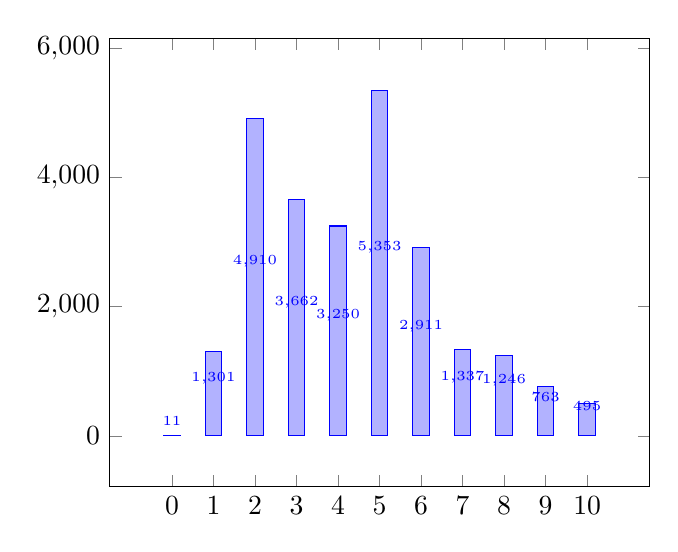
\begin{tikzpicture}
      \begin{axis}[
          bar width=6pt,
          scaled ticks=false,
          tick label style={/pgf/number format/fixed},
          ybar stacked,
          enlargelimits=0.15,
          legend style={at={(0.5,-0.15)},
            anchor=north,legend columns=-1},
          symbolic x coords={0, 1, 2, 3, 4, 5, 6, 7, 8, 9, 10},
          xtick=data,
          nodes near coords,
          every node near coord/.append style={font=\tiny},
          nodes near coords align={vertical},
        ]
        \addplot coordinates {(0,11) (1,1301) (2,4910) (3,3662) (4,3250) (5,5353) (6,2911) (7, 1337) (8, 1246) (9,763) (10, 495)};
      \end{axis}
    \end{tikzpicture}
  }
  \vspace{-2ex}
  \caption{\label{fig:distribution-rule-size}Distribution of rule sizes.}
\end{figure}



More precisely, we calculate the contribution of size of a given rule
$r$ with the following formula:

\[\frac{\mathit{rules\_per\_size}[\mathit{len(r)}]}{\mathit{max(rules\_per\_size})}\]

\noindent
, where $\mathit{len(r)}$ denotes the number of options of a rule $r$,
$\mathit{rules\_per\_size}$ encodes distribution of sizes as a
dictionary mapping sizes to number of associated rules, and
$\mathit{max(rules\_per\_size)}$ returns the maximum number of rules
for any dictionary entry. Consequently, the contribution of size is
proportional to its popularity. For example, the contribution of this
heuristic for a rule with three options would be 0.684 (=3,662/5,353)
whereas the contribution of a rule with nine options would be 0.028
(=154/5,353). Note that the measurement is normalized in the 0-1
range.

\subsubsection{Number of content options.} We empirically observed that content options are very
common. \Luc{Se for preciso temos numeros para fundamentar isso
  melhor, sao cerca de 70K contents nas 28K regras do
  dataset}\Mar{sim, isto ajuda, porem mais importante eh saber quantas
  (\%) das 28K regras tem contents.} \Luc{sao 69417 contents nas 26094 regras q utilizam contents} As consequence, we defined a
heuristic function that takes the number of content options into
account. We calculate the contribution of number of content options
with the following formula:

\begin{figure}[t!]
  \centering
  \scalebox{1.2}{  
    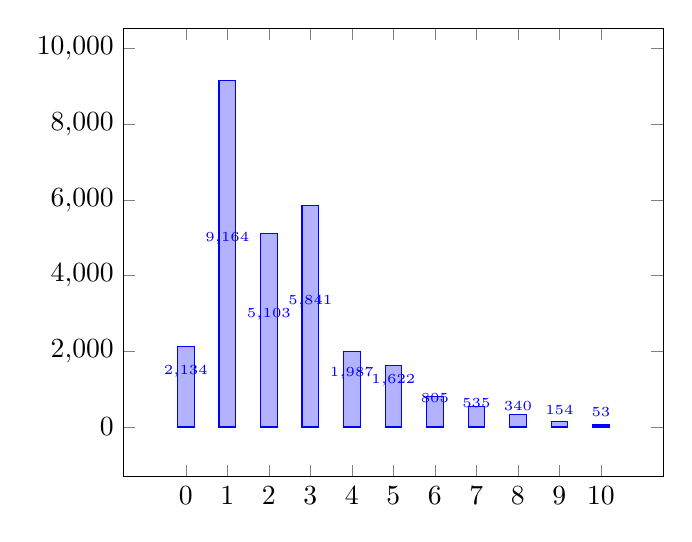
\begin{tikzpicture}
      \begin{axis}[
          bar width=6pt,
          scaled ticks=false,
          tick label style={/pgf/number format/fixed},
          ybar stacked,
          enlargelimits=0.15,
          legend style={at={(0.5,-0.15)},
            anchor=north,legend columns=-1},
          symbolic x coords={0, 1, 2, 3, 4, 5, 6, 7, 8, 9, 10},
          xtick=data,
          nodes near coords,
          every node near coord/.append style={font=\tiny},
          nodes near coords align={vertical},
        ]
        \addplot coordinates {(0,2134) (1,9164) (2,5103) (3,5841) (4,1987) (5,1622) (6,805) (7, 535) (8, 340) (9,154) (10, 53)};
      \end{axis}
    \end{tikzpicture}
  }
  \caption{\label{fig:distribution-contents}Distribution of number of
    content options.}
\end{figure}  

\[\frac{\mathit{rules\_per\_number\_of\_contents[len(r)]}}{\mathit{max(rules\_per\_number\_of\_contents)}}\]

\noindent
Note that the only difference of this formula compared to the formula
to compute contribution of size is the distribution used, which is
given by the term $\mathit{rules\_per\_number\_of\_contents}$ denoting
a dictionary of number of content options to number of rules that
contain that number of content options.

\subsubsection{Content rarity.} 
This heuristic weighs higher rules that use popular strings in content
options. For a given rule \tname{} takes the arithmetic mean of the
popularity scores of each string used in contents in that rule. More
precisely, we calculate the contribution of content rarity with the
following formula:

\[\frac{\sum_{i=1}^{N}\frac{\mathit{content\_frequency[content_i]}}{\mathit{max(content\_frequency)}}}{N}\]

\noindent
, where the term $\mathit{content_i}$ denotes the $i$-th xcontent in a
given rule, the term $\mathit{content\_frequency[\mathit{content_i}]}$
denotes the frequency of the string used in the $i$-th content, the
term $\mathit{max(content\_frequency)}$ denotes the maximum frequency
observed across all strings appearing as content parameters, and $N$
is the number of content options in a given
rule. Figure~\ref{fig:distribution-strings} shows the distribution of
the ten most popular strings in our rule dataset. To illustrate this
function, let us consider a rule with two content options, using the
strings ``GET'' and ``ID'', respectively. The contribution of that
rule for the computation of similarity score would be 0.601
(=(1+.203)/2).

\begin{figure}[t!]
  \centering
  \scalebox{1.2}{  
    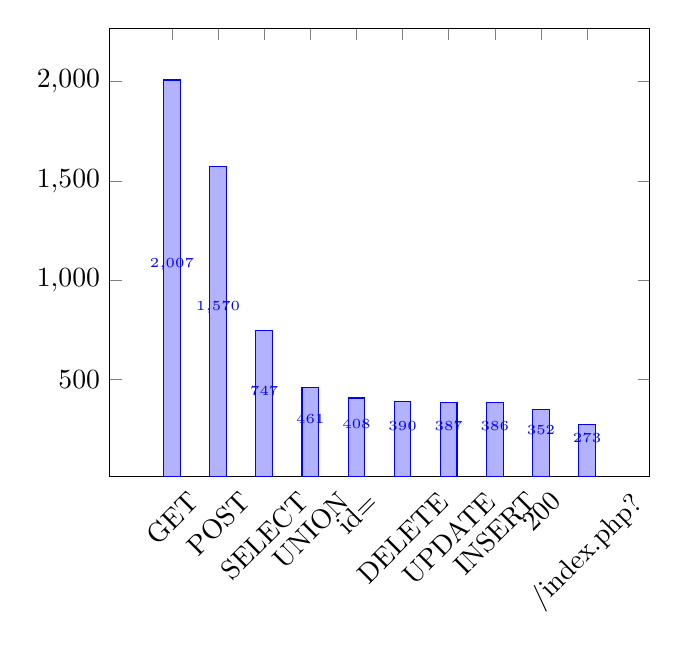
\begin{tikzpicture}
      \begin{axis}[
          bar width=6pt,
          scaled ticks=false,
          tick label style={/pgf/number format/fixed},
          ybar stacked,
          enlargelimits=0.15,
          legend style={at={(0.5,-0.15)},
            anchor=north,legend columns=-1},
          symbolic x coords={GET, POST, SELECT, UNION, id=, DELETE, UPDATE, INSERT, 200, /index.php?},
          xtick=data,
          xticklabel style={rotate=45},          
          nodes near coords,
          every node near coord/.append style={font=\tiny},
          nodes near coords align={vertical},
        ]
        \addplot coordinates {(GET,2007) (POST,1570) (SELECT,747) (UNION,461) (id=,408) (DELETE,390) (UPDATE,387) (INSERT, 386) (200, 352) (/index.php?, 273)};
      \end{axis}
    \end{tikzpicture}
  }
  \caption{\label{fig:distribution-strings}Distribution of strings
    used as parameters of content options.}
\end{figure}

\subsubsection{Frequency of content modifiers.} As previously
mentioned, \percRulesWithContent\ of Suricata rules involve content
options. Furthermore, we observed---by analyzing the dataset of
existing rules (see Section~\ref{sec:dataset-benign})---that often
these rules indicate what part of the message the content string
should be checked against.\Mar{Lucas, vc. tem dados para dar suporte a
  isto? ou seja, quantas options do tipo ``content'' possuem
  modificadores.} \Luc{das 26k regras que utilizam content, 13k delas utilizam modificadores http q sao os q nós consideramos.} For example, the
creator of the rule may want to indicate that a specific string be
present in the header of an HTTP request message. Content
\emph{modifiers} serve this purpose. For example, the modifier
\CodeIn{http\_header} in the option \CodeIn{content: ``keep-alive'';
  http\_header} states the requirement that the string ``keep-alive''
be present in the header of the message. (A keep-alive connection
attribute indicates that a single TCP connection should remain open
for multiple HTTP requests/responses.)
Figure~\ref{fig:http-header-example}

\begin{figure}[h!]
\centering
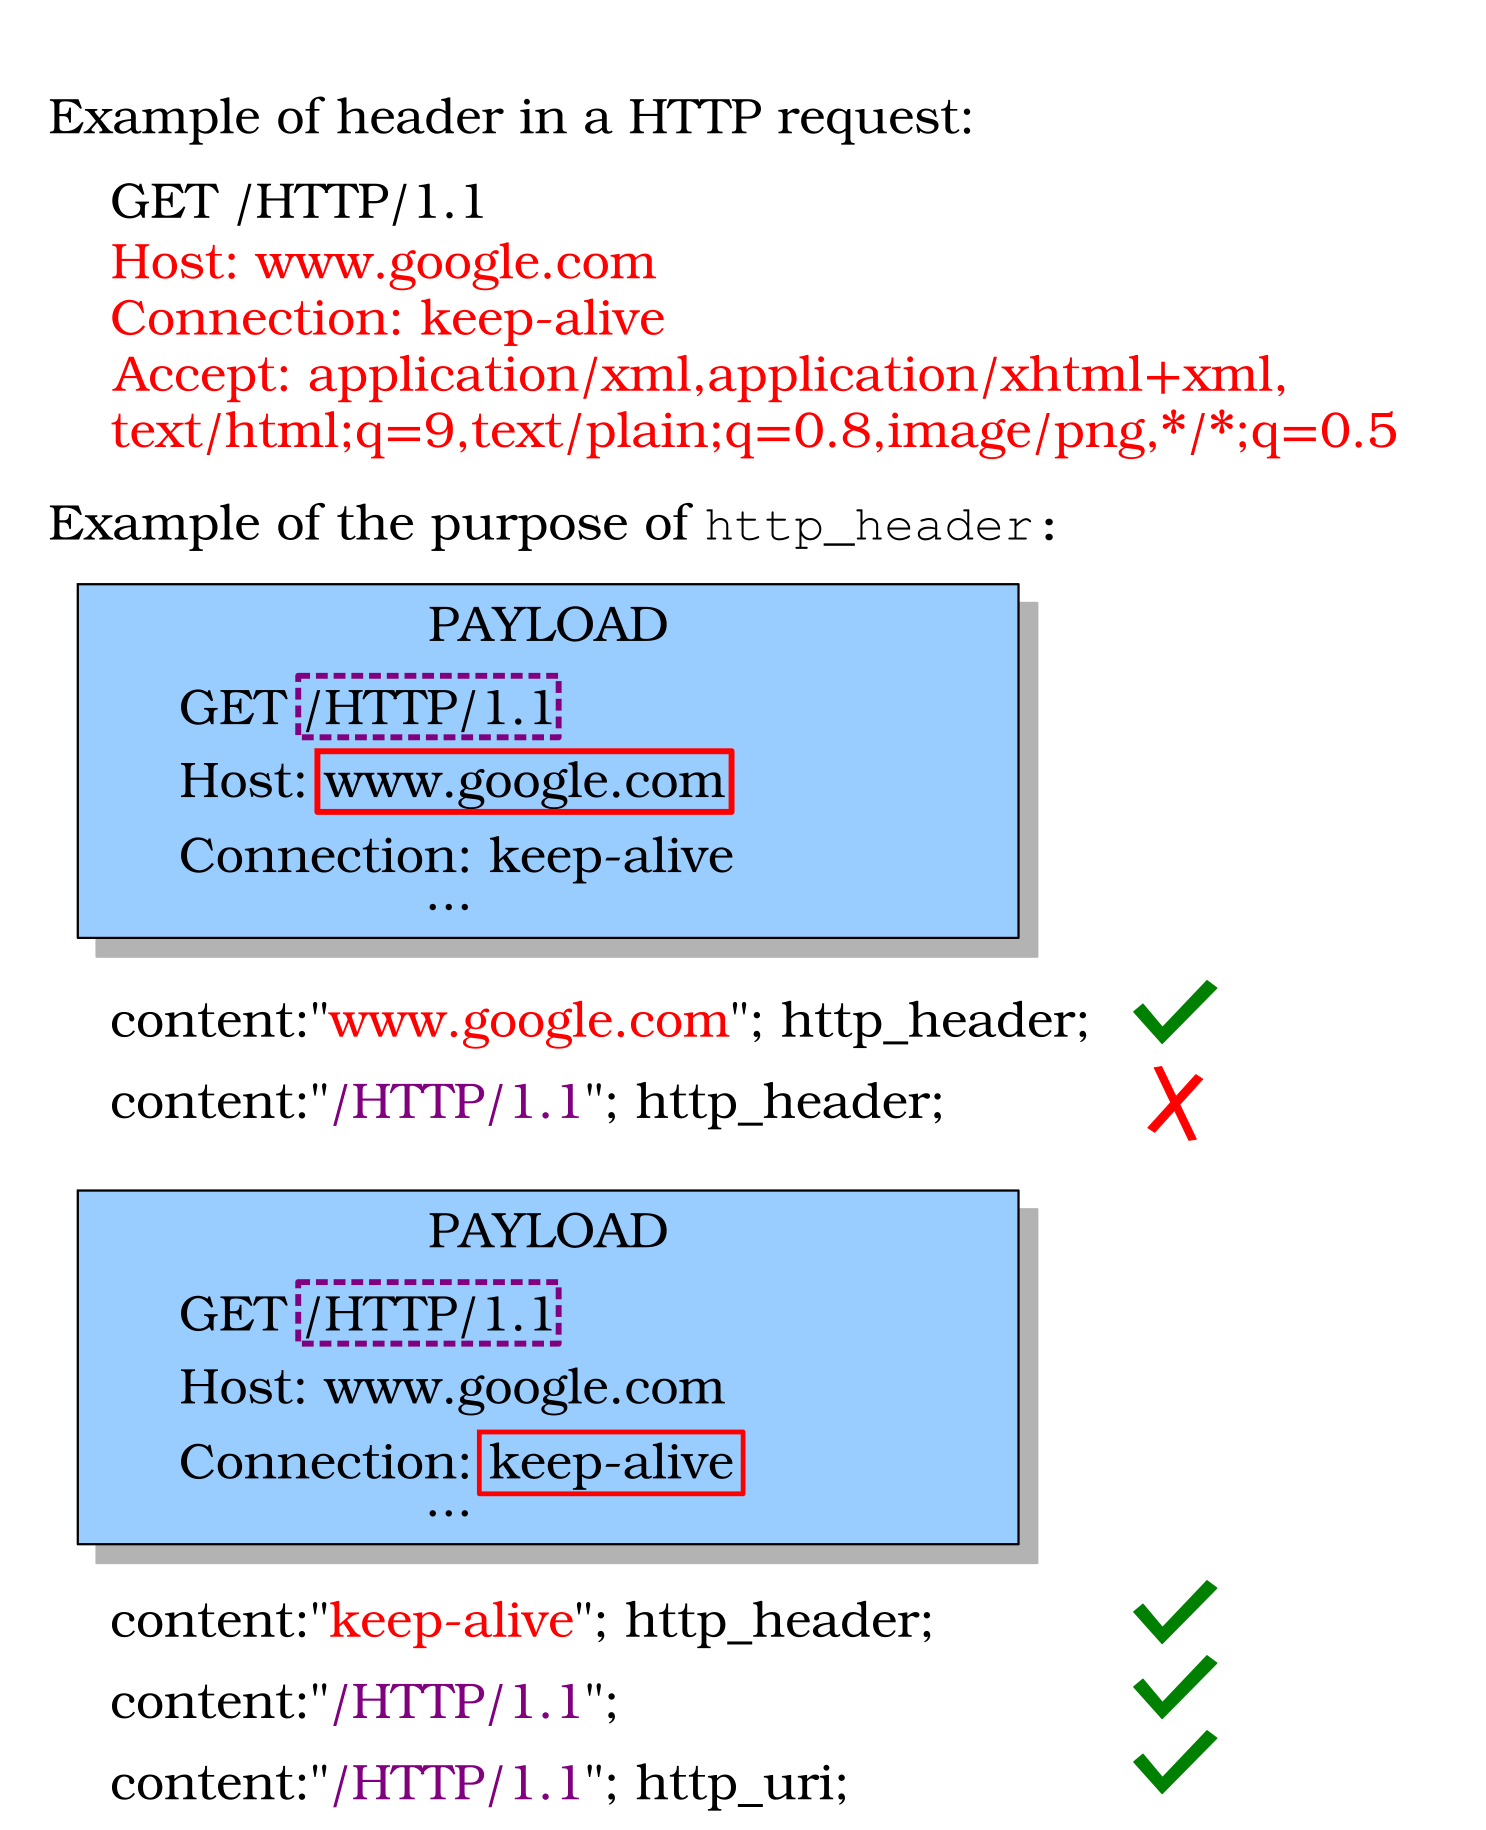
\includegraphics[scale=0.5]{figs/http_header-example.png}
\caption{\CodeIn{http\_header} example.}
\label{fig:http-header-example}
\end{figure}

%% Suricata supports content modifiers for tcp and http. \Luc{Eh possivel utilizar os modificadores em qualquer protocolo. Nós consideramos apenas tcp e http pois são os protocolos que possuem payloads legiveis, assim conseguimos saber melhor como tokenizar o conteudo. O payload de pacotes de outros protocolos, em geral, são um conjunto de bytes sem significado para nós. Existem diversos outros modificadores q não estamos considerando e q tambem permitem procurar numa determinada posição para os casos em q o conteudo do pacote n eh legivel, não citei pq não suportamos isso. Se necessário posso explicar.} Given that
%% content options often use modifiers\Mar{assumindo que eh
%%   verdade. confirmar estat. solicitada acima...},

\tname\ uses the frequency of content modifiers to discriminate rules
more or less likely to reflect actual rules. For example, historical
data indicates that content options that use the
\CodeIn{http\_connection} modifier are much less likely than content
options that use the modifier
\CodeIn{http\_uri}. Figure~\ref{fig:distribution-content_modifiers}
shows the histogram of content modifiers for http. Although content
modifiers are applicable to rules of any protocol supported by
Suricata, currently, \tname\ only supports tcp and http. These are the
protocols involving ~80\% of the rules from our dataset.

%% and
%% (2) the payload of messages of different protocols are not as
%% segmented as the case of tcp and http. Consequently, rule writers do
%% not refer to specific parts of the payload as often as the task o and
%% more challenging for

Similarly to the the previous heuristic functions, this function uses
the frequency of content modifiers to calibrate the score of each
rule. More precisely, we compute this function with the following
formula:

\[\frac{\sum_{i=1}^{N}g(i)}{N},~g(i)=\frac{\sum_{j=1}^{M_i}\frac{\mathit{modifier\_frequency[modifier_{ij}}]}{\mathit{max(modifier\_frequency)}}}{M_i}\]

\noindent
, where $N$ is the number of contents options, $g(i)$ is the
contribution of content option $i$ to the score,
$\mathit{modifier\_frequency[modifier_{ij}}]$ denotes the popularity
of a modifier $j$ to content option $i$,
$\mathit{max(modifier\_frequency)}$ refers to the modifier with
maximum popularity (for normalization), and $M_i$ is the number of
content modifiers that could access the string associated with content
$i$.


%% \Mar{Qual o rationale para considerar as varias
%%   alternativas de acesso ao inves de apenas a alternativa que eh mencionada?}0
%%   \Luc{Vc está supondo que as regras que geramos incluem os modificadores e que deveriamos pontuar somente de acordo com os que estão presentes? Não eh o caso. A ideia aqui basicamente eh: se um certo content do payload está numa posição q eh muito verificada nas regras, possivelmente esse content eh mais relevante do q outro q está numa posição q raramente eh verificada. Para avaliar isso nós só precisamos saber quantas vezes os modificadores que acessam essas posições aparecem no dataset.}
%%   \Luc{Uma coisa que pensei agora foi de considerar apenas o modificador mais comum entre aqueles que acessam a posição de um content. Como a pontuação de um content eh dado pela media das ocorrencias dos modificadores que conseguem acessá-lo, se houver um modificador muito comum e varios modificadores raros a pontuação dada será baixa.}
                                                                             
%% \Luc{$M_i$ eh o numero de modificadores que podem referenciar a posição em q se encontra o $content_i$}\Mar{isto eh confuso. vc. esta dizendo que
%%   o mesmo content pode ter mais de um modificador? ou a string poderia
%%   ser acessada por mais de um modificador. se for este o caso,
%%   sinceramente, achei isto bem confuso. afinal, a regra jah indica
%%   qual o modificador foi escolhido para acessar a string.}.\Luc{Cada content em uma regra só pode possuir um modificador para indicar a posição onde ele deve ser procurado. Entretanto sim, uma "string poderia
%%   ser acessada por mais de um modificador", foi o caso daquele exemplo com o http\_header.} \Luc{M eh
%%   o numero de modificadores associados a cada content. Temos
%%   content[1], content[2], ..., content[N]. Cada um desses contents tem
%%   modificadores associados content[i][1], content[i][2], ...,
%%   content[i][M].}\Mar{Lucas, e se nao houver modificador algum em um
%%   content. a frequencia seria 0, correto?} \Luc{Sim}


\begin{figure}[t!]
  \centering
  \scalebox{1.2}{
    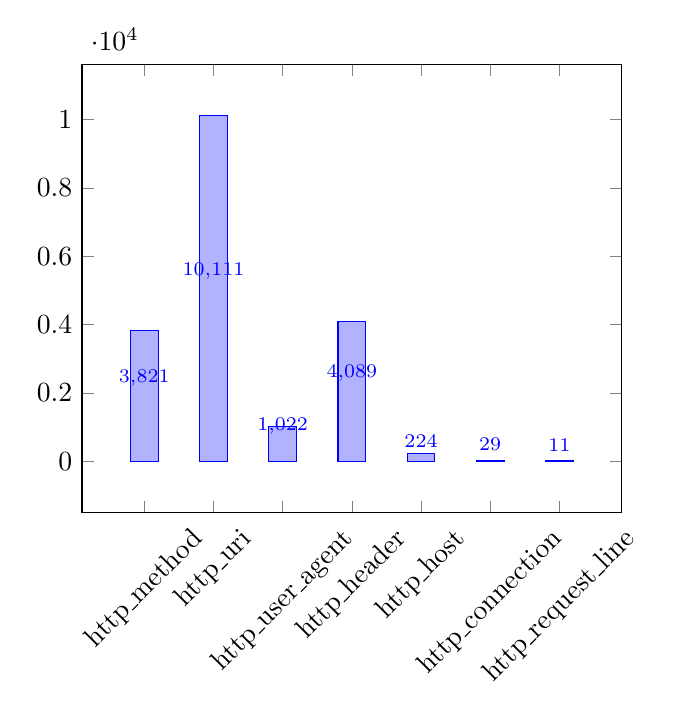
\begin{tikzpicture}
      \begin{axis}[
          ybar stacked,
          enlargelimits=0.15,
          legend style={at={(0.5,-0.15)},
            anchor=north,legend columns=-1},
          %          ylabel={\#rules},
          symbolic x coords={http\_method, http\_uri, http\_user\_agent, http\_header, http\_host, http\_connection, http\_request\_line},
          xtick=data,
          xticklabel style={rotate=45},          
          nodes near coords,
          every node near coord/.append style={font=\scriptsize},        
          nodes near coords align={vertical},
        ]
        \addplot coordinates {(http\_method,3821) (http\_uri,10111) (http\_user\_agent,1022) (http\_header,4089) (http\_host,224) (http\_connection,29) (http\_request\_line,11)};
      \end{axis}
    \end{tikzpicture}
  }
  \vspace{-2ex}
  \caption{\label{fig:distribution-content_modifiers}Content modifiers
    frequency.}
\end{figure}


%\Mar{what about ``none'' (no modifier)?}}
%  \Luc{Uma regra pode sim ter contents sem modificadores, mas isso n
    %% vem ao caso aqui. Nessa heuristica toda string do payload vai ter
    %% associada a ela os modificadores q podem acessar a sua
    %% posição. Portanto, não vai existir o caso de não haver
    %% modificador. Atenção: isso não quer dizer q as regras q geramos
%% incluem os modificadores, elas n incluem.
%\Luc{Inclui esse modificador pq ele tambem pode acessar o campo Request URI. Isso eh um problema? O http\_uri eh o modificador mais comum, mas o fato de haver o modificador http\_request\_line que tambem accessa a mesma posição faz com que o fitness maximo seja 0.5, pois a ocorrencia de http\_request\_line eh irrelevante no calculo.}
    
Consider a rule containing the option \CodeIn{content:
  ``/HtmlAdaptor''}. The contribution of this option to the score of
the rule that uses it would be $0.5$
(=$\frac{10,111+11}{10,111*2}$). The value of $M_i$ for this case is 2
as the field of the HTTP message \CodeIn{Request URI}---holding the
string ``/HtmlAdaptor''---can be accessed through the modifiers
\CodeIn{http\_uri} and \CodeIn{http\_request\_line}. The relatively
high heuristic value given to this option suggests it is a plausible
option to be used in rules---the string used in the content option
(``/HtmlAdaptor'') is stored in a specific field of the HTTP message
(\CodeIn{Request URI}) and can be accessed by two content modifiers,
namely (\CodeIn{http\_uri} and \CodeIn{http\_request\_line}). For the
option \CodeIn{content: ``keep-alive''}, either the modifier
\CodeIn{http\_header} or the modifier \CodeIn{http\_connection} could
be used to locate the string ``keep-alive'' stored in the field
\CodeIn{Connection} (see Figurgure~\ref{fig:http-header-example}). Consequently, for this
case, the contribution of modifiers to this content option would be
$0.2$ (=$\frac{4089+29}{10111*2}$). Assuming that both options are
used in a rule, the aggregated contribution of this heuristic function
would be 0.35 (=(0.2+0.5)/2).

%% \section{Modificadores}É possivel deixar que uma regra verifique todo o payload do pacote em busca de um match com um content ou especificar partes do payload onde esse content deve ser procurado. Essa definição é feita utilizando os chamados modificadores de content, eles adicionam mais detalhes/informações sobre a detecção de um determinado content. Os modificadores que estamos considerando são validos apenas para regras dos protocolos tcp e http.

%% Exemplo do payload "cru" de um pacote http:\\
%% Aqui, todas as informações do pacote estão juntas.

%% \begin{figure}[h!]
%%   \lstinputlisting[language=C,numbers=none,keywords={content}]{http-example.payload}
%% \end{figure}

%% O mesmo payload interpretado pelo Wireshark:\\
%% Aqui, o wireshark interpreta as informações dos pacotes e as divide para melhor visualização e entendimento.

%% \begin{figure}[H]
%%   \lstinputlisting[language=C,numbers=none,keywords={content}]{http-example-wireshark.payload}
%% \end{figure}

%% O que o suricata faz eh identificar os campos e seus valores e com isso permite que as regras façam referencia direta a eles. Por exemplo, na figura do payload "cru" não conseguimos identificar facilmente oq eh o "Request URI Path:", já na segunda figura isso está explícito.

%% Eu disse que o "GET" estava associado tambem ao http\_header, mas não está, me enganei. Mas sim, pode haver interseção entre os campos que dois ou mais modificadores referenciam. O seguinte trecho do payload é acessado pelo modificador http\_header:

%% \begin{figure}[H]
%%   \lstinputlisting[language=C,numbers=none,keywords={content}]{http-header.payload}
%% \end{figure}

%% Entretando, tambem existem os modificadores http\_host,
%% http\_accept\_enc, http\_connection e http\_accept que permitem
%% acessar diretamente cada uma das linhas acima.

%% \Mar{Lucas, use uma regra concreta com a regra da Secao 3.3 (assumindo
%% que vai mante-la) e mostre como eh feito o calculo da regra desta
%% funcao heuristica para regra inteira.}\\
%% \Luc{-------------}



%% A avaliação que fazemos aqui pontua um dado content de acordo com quantas vezes o campo em que ele se encontra eh referenciado nas regras. Por exemplo, vamos supor que o tokenizer produziu a opção content: "/HtmlAdaptor". Essa string pertence ao campo "Request URI:". Esse campo pode ser acessado pelo modificador http\_uri. O tokenizer associa o content a esse modificador. 
%% Posteriormente, esse content vai receber uma pontuação
%% correspondente a popularidade desse modificador:\\


%% A multiplicação por 1 no denominador eh referente a quantidade de
%% modificadores que estão associadas a esse content.\Luc{O correto eh ser dividido pela quantidade de modificadores. Atualizei a formula para tentar representar isso. Considere que no exemplo acima o content pudesse ser acessado por mais de um modificador. A pontuação dele então seria $\frac{10,111+x}{10,111*1}$ > 1. Para manter a pontuação entre 0-1, o certo nesse caso seria fazer $\frac{10,111+x}{10,111*2}$}\Mar{nao foi isto
%%   que vc. disse acima, Lucas. foi dito que N (=2) era o numero de
%%   contents e o exemplo acima tem apenas 1 content.}  

%% Content options are
%% associated with specific packets fields\Mar{or modifiers?}.\Mar{why
%%   GET is associated with http\_method and http\_header?}\Mar{are all
%%   content associated with one or many fields or positions in a packet?
%%   can you give examples other than GET to explain this? if yes,
%%   shouldn't this be discussed before? Maybe Section 2.3?}\Mar{Also, it
%%   is important to justify (to explain rationale)---how is it different
%%   from counting rarity?}


%% Esse componente pontua um content de acordo com o campo ao qual ele pertence no pacote. Contents que pertencem a campos mais comuns (campos que são mais referenciados nas regras) recebem maior pontuação.
%% Modificadores diferentes podem acessar campos iguais em um pacote. Por
%% exemplo os modificadores http\_method e http\_header, o http\_method
%% acessa apenas o metodo do pacote http, mas o http\_header acessa todo
%% o cabeçalho (incluindo o proprio metodo). Com isso, a string "GET"
%% receberia a pontuação correspondente a esses dois modificadores.


\section{Evaluation}

This section evaluates the precision and efficiency of \tname{}.

\subsection{Objects of Analysis}
\label{sec:dataset-benign}

Table~\ref{table:attacks} shows the attacks we considered in our
evaluation. These attacks cover different protocols and features of
\tname{}. Column ``Name'' shows the name of the attack, column
``Protocol'' shows the protocol name, and column ``Ground Truth''
shows the options of the rule that captures the attack.

\vspace{1ex}
\noindent
\textbf{Malicious traffic.}~Nikto?\Fix{where do these
  attacks/messages come from?}
  \Luc{Nós executamos um servidor http (Apache2) numa maquina e executamos o Nikto em outra maquina atacando o servidor http. Capturamos o trafego q chegava ao servidor e eh ele q estamos utilizando.}

\vspace{1ex}
\noindent
\textbf{Benign traffic.}~\tname{} uses public databases storing benign
traffic for all protocols covered by Suricata (see
Figure~\ref{fig:distribution-rules-protocol}). We used two datasets of
positive traffic. The Bigflows.pcap dataset is part of the
TcpReplay~\cite{tcpreplay} open source project. This dataset includes
real network traffic on a busy private network access point to the
Internet. According to the TcpReplay web site ``This capture is much
larger and has a smaller average packet size than the previous capture
(smallFlows.pcap). It also has many more flows and different
applications.''. In addition to the Bigflows.pcap dataset, we also
used datasets of normal traffic made available by Stratosphere
Lab~\cite{stratosphere-normal}.

\vspace{1ex}
\noindent
\textbf{Ground Truth.}~The rules that detect those attacks were
obtained from the Emerging Threats Open
Ruleset~\cite{emerging-threats-open}.

%% Note from Figure~\ref{fig:overview} that the positive traffic is an
%% input to the technique. The negative non-malicious traffic, however,
%% is not.


\begin{table*}[h]
  \caption{\label{table:attacks}List of attacks.\Mar{Guilherme, por
      favor, adicione mais ataques aqui...}}
  \centering
  \begin{tabular}{lll}
    \toprule
    \multicolumn{1}{c}{Name} &
    \multicolumn{1}{c}{Protocol} &
    \multicolumn{1}{c}{Groud Truth} \\
    \midrule     
    Ping Scan \MyComment{& single} & ICMP \MyComment{& Discovers
      active hosts in a network} & \scriptsize{dsize:0; itype:8;} \\
    Black Nurse \MyComment{& multiple} & ICMP \MyComment{& Denial of Service} & \scriptsize{itype:3; icode:3; detection\_filter:track by\_dst, count 250, seconds 1;}\\
    Ping Flood  \MyComment{& multiple} & ICMP \MyComment{& Denial of Service} & \scriptsize{itype:8; icode:0; detection\_filter:track by\_src, count 30, seconds 1;}\\  
    Port Scan \MyComment{& single} & TCP \MyComment{& Discovers open ports in a host} & \scriptsize{flags: A; ack: 0;dsize: 0;} \\
    SYN Flood \MyComment{& multiple} & TCP \MyComment{& Denial of Service} & \scriptsize{flags: S,12; threshold: type both, track by\_dst, count 5000, seconds 5;}\\
    UDP Flood \MyComment{& multiple} & UDP \MyComment{& Denial of Service} & \scriptsize{fragbits:M; threshold: type both, track by\_dst, count 5000, seconds 5;} \\
    \bottomrule
  \end{tabular}
\end{table*}



\subsection{Methodology}

\subsubsection{Attack reproduction.} \tname{} requires the attack to
be replayed in order to check whether or not the rule it generates
captures the attack.  See function $\mathit{isPlausible}$, used in the
minimization algorithm from Section~\ref{sec:minimization}. For all
attacks listed on Table~\ref{table:attacks}, we found scripts
available on the web to replay the attacks. For example, the SYN Flood
attack can be replayed with hping3~\cite{hping3}, using the following
command: \CodeIn{hping3 -d 80 -w 64 -S -p 80 --flood --rand-source
  <IP>}. With the script to reproduce the attack, we executed the
following steps to obtain ``pcap'' files, which abstracts network
messages~\cite{pcap}, to run \tname:~1)~instantiate the script (\eg{},
define the IP, for the example above), 2)~execute the script,
3)~monitor the traffic with the wireshark network
monitor~\cite{wireshark-net-monitor}.

Recall that Suricata is invoked multiple times in the process of
minimizing the rule (see Section~\ref{sec:minimization}). Suricata
supports a feature to process ``pcap'' files, enabling very efficient
performance compared to processing actual network messages.
  
\Gui{
O procedimento que já tínhamos representa a etapa de treinamento. Toda aquela parte que foi explicada na apresentação para os outros professores e descrito no paper. Descreverei novamente pra confirmar, e também foi adicionado uma pequena etapa.

TREINAMENTO

->Syrius recebe como input um pcap contendo o ataque (no caso de ataques com content, usamos ataques do Nikto), um pcap benígno (usamos o bigflows.pcap) e um pcap contendo as variações de ataque (isso pode ser otimizado unificando com o pcap de ataque, mas por agora está assim)
->É gerado a regra máxima através do tokenizer e engenharia reversa.
->Syrius remove UM content de uma regra da lista de regras atuais (inicialmente apenas a regra máxima) e checa se a regra criada já existe na lista. Se não, a regra é adicionada à lista de regras-não-testadas. Syrius faz isso duas vezes por regra, para todas as regras da lista.
->A lista de regras-não-testadas é inicializada no suricata e então o rodamos com o pcap benígno de treinamento (75porcento do total). Verificando no arquivo de log do suricata, caso a regra alerte, ela é removida da lista. As regras restantes vão para a lista de regras atuais.
->Quando não houver alterações, retornamos a lista com todas as regras que deram certo.
->Opcionalmente, ainda rodamos no final uma variação de ataque (no momento apenas um pacote devido ao número limitado que temos do ataque). Ao contrário do método com pacotes benígnos, se a regra NÃO alertar, ela é removida.
->Calculamos o fitness de cada regra e ordenamos de acordo com o fitness resultante. Esta lista ordenada é o fim do treinamento.

TESTE

->Inicializamos a lista de regras ordenadas no suricata e rodamos o pcap benígno de teste (25porcento restantes) para cálculo do precision. O cálculo ficou basicamente, por regra: [100 - (numero-de-alertas/total-de-pacotes)]

->Inicializamos a lista de regras ordenadas no suricata e rodamos o pcap com variações de ataque (caso a etapa opcional ocorrer, não usamos aquele pacote especifico) para cálculo do recall. O cálculo ficou basicamente, por regra: [(100/total-de-pacotes) * n-alertas].

->Por final calculamos o F1 Score por regra: [2*((precision*recall)/(precision+recall))]

->O teste retorna um csv contendo a lista de regras ordenadas com seus respectivos precision, recall e f1 score.
}

%% \Gui{We are using the bigflows.pcap provided by tcpreplay on http://tcpreplay.appneta.com/wiki/captures.html "This is a capture of real network traffic on a busy private network’s access point to the Internet"
%%  }

%% \Luc{entrada: utilizamos a ferramenta hping3 para executar o ataque em um alvo arbitrario dentro da rede (n ha necessidade de haver um alvo real para executar o hping3) e capturamos o trafego gerado com o wireshark. o comando utilizado foi:\\*
%% \texttt{\# hping3 -d 80 -w 64 -S -p 80 --flood --rand-source 192.138.1.115} \\*
%% que envia pacotes de 80 bytes (-d 80), com a flag SYN habilitada (-S), tamanho de janela de 64 bytes (-w 64), direcionados a porta 80 (-p 80). A flag --flood indica q o hping3 vai enviar os pacotes o mais rápido possível. a flag --rand-source indica que cada pacote vai ter um ip de origem aleatorio. 192.138.1.115 é o alvo.\\*
%% O trafego armazenado contem 40 mil pacotes SYN, enviados no intervalo de 1 segundo,  pegamos uma amostra de 20 desses pacotes para representar o flood e servir como entrada.\\*
%% O wireshark armazena os pacotes no formato pcap, utilizamos a ferramenta tcpreplay para reproduzir o trafego com o comando:\\*
%% \texttt{\# tcpreplay --pps 200 --intf1=wlp2s0 Datasets/syn-flood-sample.pcap}\\*
%% Nesse caso, estamos enviando os pacotes armazenados em \texttt{Datasets/syn-flood-sample.pcap} a uma taxa de 200 pacotes por segundo (\texttt{-pps 200}) utilizando a interface wlp2s0 (\texttt{--intf1 wlp2s0})\\* 
%% Há diferenças entre os pacotes na opção ack.\\* 
%% Por que 20? Apenas para gerar a regra mais rapidamente, poderia ser qualquer valor maior ou menor. No final, o parâmetro \texttt{count} da opção \texttt{threshold} vai ser alterado pelo adm da rede.\\*
%% Intervalo de reprodução: 0.005 segundo

%% }

%% \Fix{any other detail we should consider?}

\subsection{Precision}

\Fix{}

\subsection{Efficiency}

\subsection{Threats to Validity}

External Validity. \Fix{elaborate ...how popular are Suricata/Metasploit?}

\section{Related Work}

\Fix{...}

\section{Conclusions}

\Fix{...}

%% \section*{Acknowledgments}
%% This work is partially supported by RNP grant number 002951.


\bibliographystyle{ACM-Reference-Format}
\bibliography{references}

\end{document}
\endinput
%%
%% End of file `sample-sigconf.tex'.
